\documentclass[11pt]{article}

\usepackage{amsmath,amssymb,amsfonts,enumitem,graphicx}

\setlength{\topmargin}{-.5in} \setlength{\textheight}{9.25in}
\setlength{\oddsidemargin}{0in} \setlength{\textwidth}{6.8in}

\begin{document}

\Large

\noindent{\bf Computer Graphics\hfill Midterm}


\medskip\hrule
\begin{enumerate}[start=0]

\item Which handles \textbf{alpha blending}: the graphics \textit{engine} or the graphics \textit{API} (i.e. OpenGL)?
\vspace*{50px}

\item What does \texttt{setAnimationFrame} do that a loop and \texttt{setInterval} cannot?
\vspace*{50px}

\item Please fill in the empty boxes on the following diagram of a \textbf{graphics pipeline}.
\vspace*{25px}

\begin{figure}[h!]
  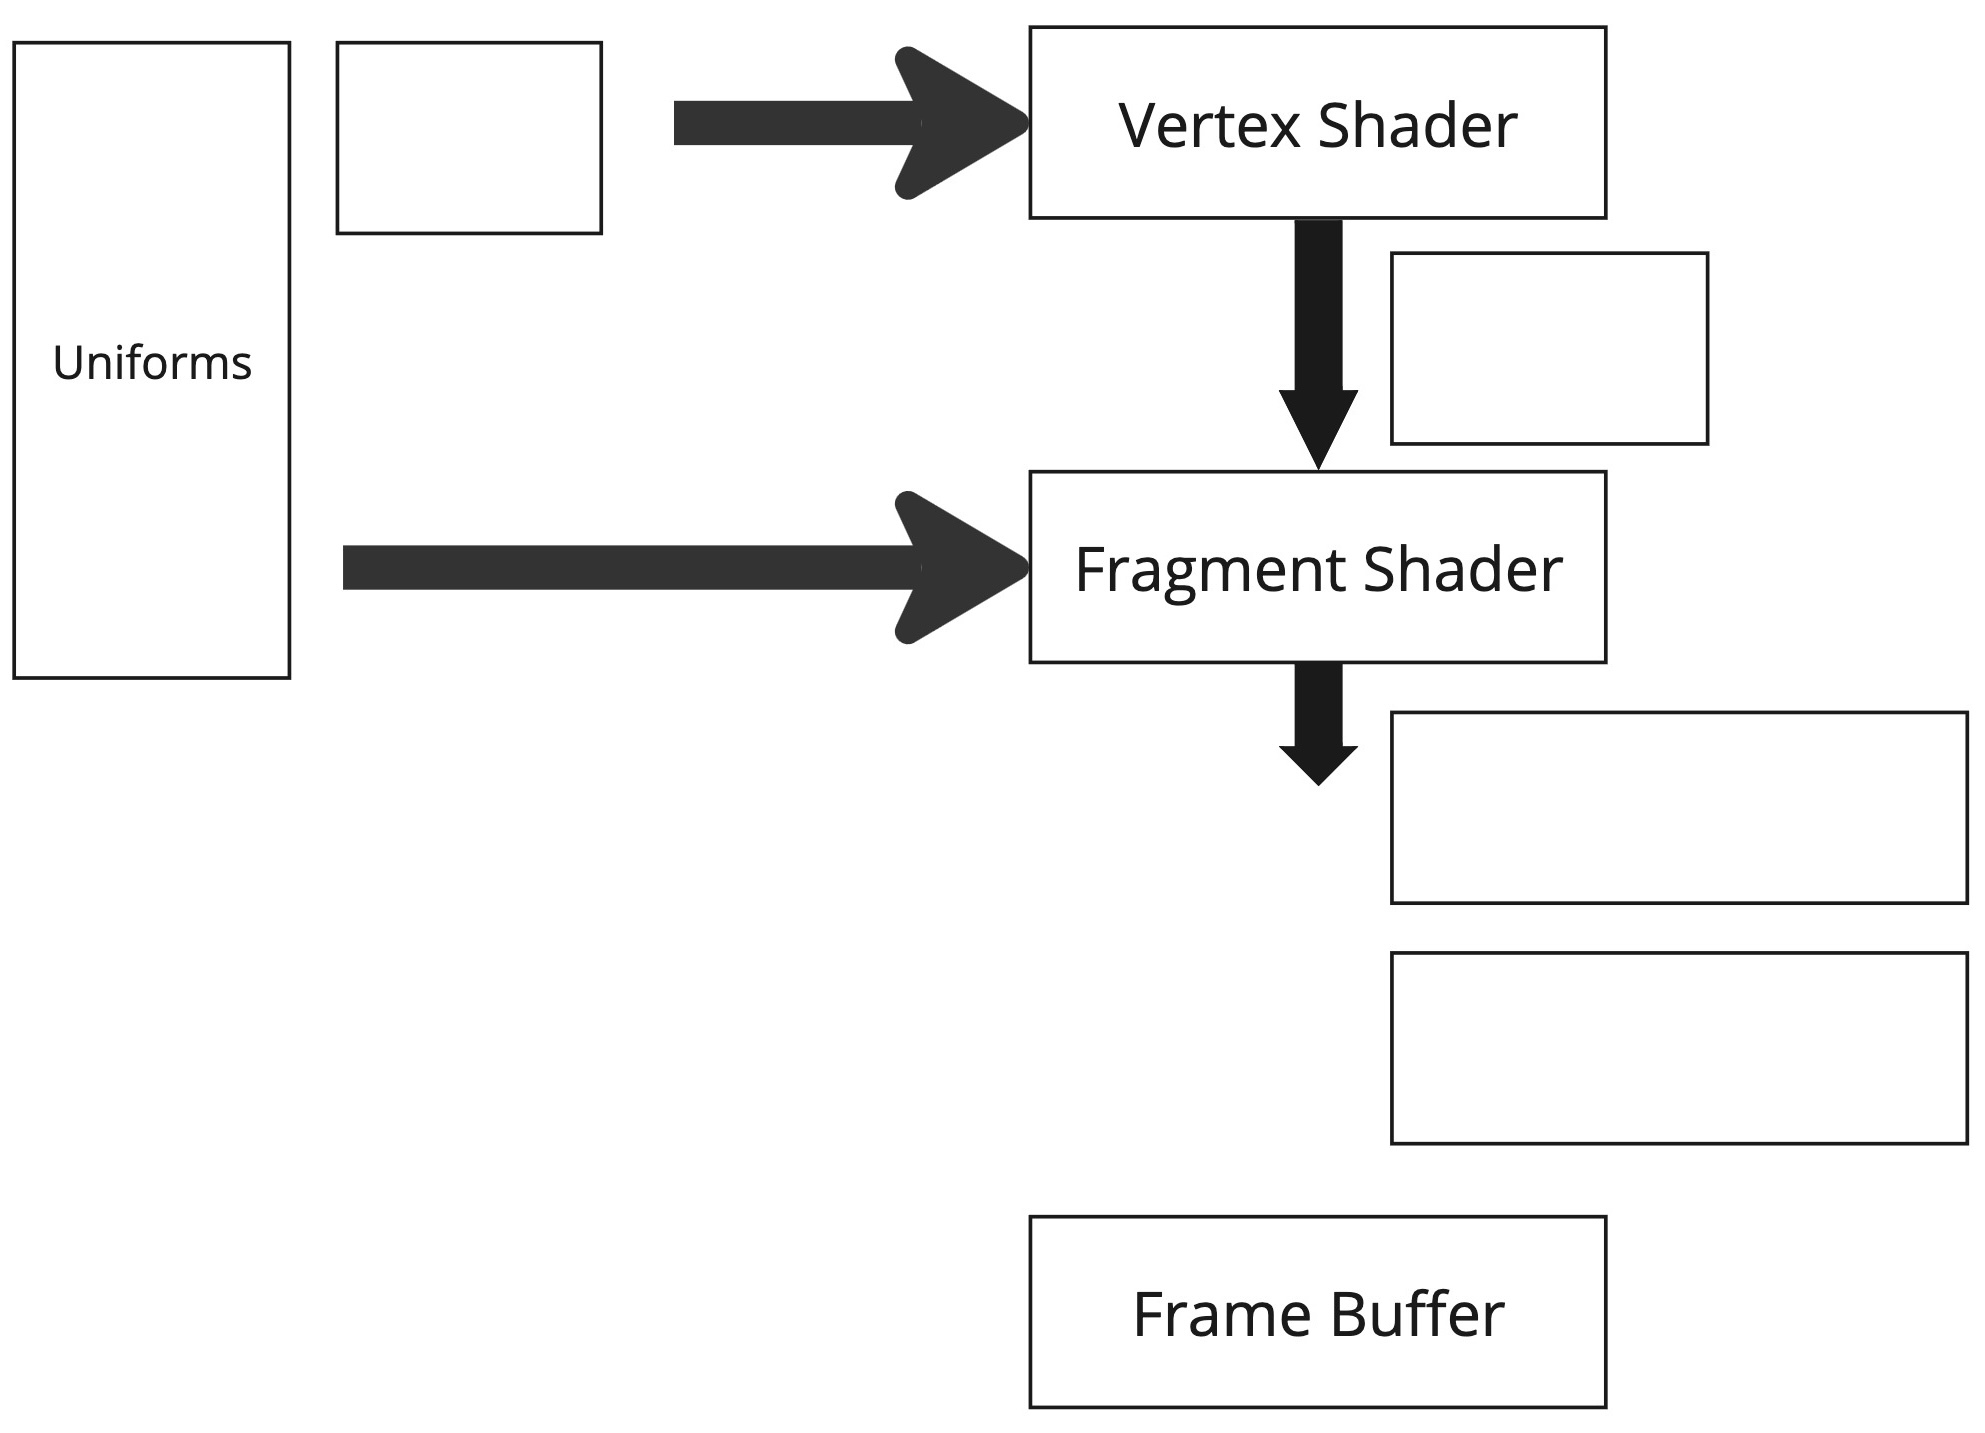
\includegraphics[width=\linewidth]{pipeline.jpg}
\end{figure}

\newpage

\item Which of these operates on \textit{interpolated} data (circle one)?
\begin{center}
$%
\begin{array}{ccccc}
\textbf{Vertex shader}
\\
\vspace*{1px}
\\
\textbf{Fragment shader}
\\
\vspace*{1px}
\\
\end{array}%
$
\end{center}

\item In addition to the frame buffer, what other buffer is modified by a fragment shader?
\vspace*{25px}

\item What is a \textbf{draw call}?
\vspace*{25px}

\item How are a vertex buffer and an index buffer related?
\vspace*{25px}

\item Name three different \textbf{render modes}.
\vspace*{25px}

\item Give three examples of \textbf{affine} transformations.
\vspace*{25px}

\item The \textbf{depth test} must be configured to properly for WebGL to compare depths. What are 3 different depth test configurations you can use?
\vspace*{25px}

\item Given the coordinate $(x, y, z)$, what is the corresponding \textbf{homogeneous coordinate} before any other transformations are applied?
\vspace*{25px}

\item Why do we need to transform into homogeneous coordinates at all?
\vspace*{25px}

\item The \textbf{Model Matrix} transforms between what two spaces?
\vspace*{25px}

\item The \textbf{Projection Matrix} contains two transformations: what are they?
\vspace*{25px}

\item What is a \textbf{spritesheet}?
\vspace*{35px}

\item What is \textbf{clip-space} (hint: it is NOT $[0, 0]x[1,1]$)?
\vspace*{25px}

\item What six planes define a frustum?
\vspace*{25px}

\item How do we specify \textbf{per vertex} data?
\vspace*{25px}

\item If your vertex buffer contains 636 elements, how many elements will your color buffer contain?
\vspace*{25px}

\item How do we specify data \textbf{between} vertices?
\vspace*{25px}

\item True or false: ST-coordinates and UV-coordinates are the same thing (circle one).
\begin{center}
$%
\begin{array}{ccccc}
\textbf{True}
\\
\vspace*{1px}
\\
\textbf{False}
\\
\vspace*{1px}
\\
\end{array}%
$
\end{center}

\item Name two configuration options on a \textbf{sampler}.
\vspace*{25px}

\item What is the difference between a \textbf{pixel} and a \textbf{texel}?
\vspace*{25px}

\item If a texture's dimensions at mip level 0 are \texttt{512x512}, what are the dimensions at mip level 1?
\vspace*{25px}

\item What is the difference between bilinear and trilinear filtering?
\vspace*{25px}

\item True or false: multiplying a UV by a parameter in a fragment shader results in a \textbf{dependent texture read} (circle one).
\begin{center}
$%
\begin{array}{ccccc}
\textbf{True}
\\
\vspace*{1px}
\\
\textbf{False}
\\
\vspace*{1px}
\\
\end{array}%
$
\end{center}

\item Given the blending function, $b(S, D) = S \cdot sW + D \cdot dW$, what are $S$ and $D$?
\vspace*{25px}

\newpage

\item This is a five part question: \textbf{please answer all five parts}. You have a \texttt{100x100} texture filled with values $(x, y, 0)$ at every pixel coordinate $(x, y)$. For example, this means that the value at pixel coordinate $(42, 10)$ is $(42, 10, 0)$. The value at pixel coordinate $(1, 0)$ is $(1, 0, 0)$, and so on. 
\vspace*{15px}

What UV coordinate would you need to use to sample the texture at pixel coordinate $(12, 46)$?
\vspace*{55px}

Given the UV coordinate $(0.555, 0.555)$, what value would be returned using the \texttt{gl.NEAREST} filter mode?
\vspace*{55px}

Given the UV coordinate $(0.555, 0.555)$, what value would be returned using the \texttt{gl.LINEAR} filter mode?
\vspace*{55px}

Given the UV coordinate $(1.1, 1.1)$, what value would be returned using the \texttt{gl.NEAREST} filter mode with wrapping \texttt{gl.CLAMP}?
\vspace*{55px}

Given the UV coordinate $(1.1, 1.1)$, what value would be returned using the \texttt{gl.NEAREST} filter mode with wrapping \texttt{gl.REPEAT}?


\end{enumerate}
\end{document} 